Users must be logged in the system to use its services.
During the login process users must choose the type of account (user or taxi), insert the username and the password. If everything is fine, then the users are redirected to their account page.
In the 'user login' page, guests can be redirected to the 'registration' page.

\subparagraph{Use case}
\noindent
    \begin{center}
        \begin{longtable}{| l | p{0.6\textwidth} |}
            \hline
            Actor & Registered user \\
            \hline
            Goal & Goal~\ref{g-manage}
            \\
            \hline
            Input condition & A user chooses to login \\
            \hline
            Event Flow & 
                \begin{enumerate}
                	\item On the main page of the application the user clicks the 'login' button;
                	\item The user fills the form presented with his credentials;
                	\item The user sends the form to the system for the credentials verification.
            	\end{enumerate}
            \\
            \hline
            Output condition & The system tells the user he is successfully logged in and displays the user account page. \\
            \hline
            Exception & The user inserts wrong credentials (username/e-mail and password) and the system notifies him presenting the 'login' page again with an error message. \\
            \hline
        \end{longtable}
    \end{center}


\subparagraph{Functional requirements}
\noindent
	\begin{itemize}
		\item In the 'user field', users can insert the email or the username chosen during the registration phase.
		\item If a user makes a mistake while inserting the credentials, a suggestion field in the page pops up, and it will help the user to recover his credentials.
		\item After inserting the password for 3 times, the account freezes and the user receives an e-mail with the instructions to unfreeze the account.
		\item The 'username field' is case insensitive.
	\end{itemize}


\begin{figure}[H]
    \centering
    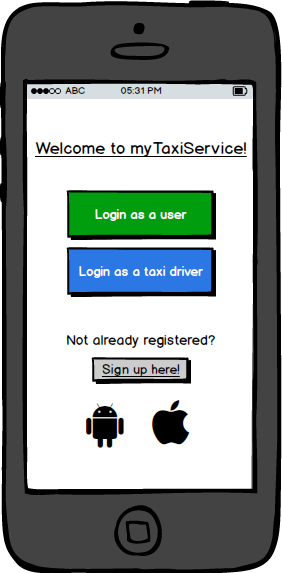
\includegraphics[width=5cm]{./Mockups/Login.png}
    \caption{Login page of the mobile application}
\end{figure}

\begin{figure}[H]
    \centering
    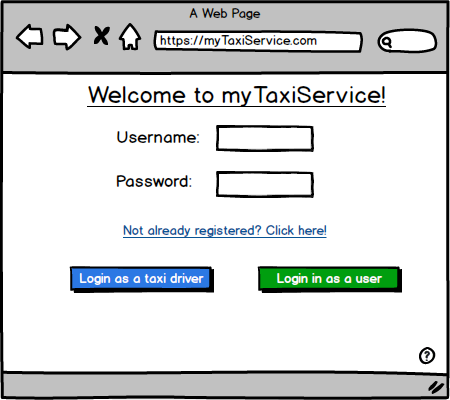
\includegraphics[width=\textwidth]{./Mockups/LoginWeb.png}
    \caption{Login page of the web application}
\end{figure}